\documentclass[12pt]{article}

\setlength{\parindent}{0pt}
\setlength{\parskip}{2mm}

\usepackage{geometry}
 \geometry{
 letterpaper, left=20mm, right=20mm,  top=20mm,
 }
\usepackage{graphicx}
\graphicspath{ {graphics/} }
\usepackage{amssymb}

%%%%%%%%%%%%%%%%%%%%%%%%%%%%%%%%%%%%%%%%%%%%%%%%%
\title{Transmission Protocol --- iCRAB}
%%%%%%%%%%%%%%%%%%%%%%%%%%%%%%%%%%%%%%%%%%%%%%%%%

\author{
	Noah Strong
}

\date{\today\ -- v1.0-wip}

\begin{document}

\maketitle

%\tableofcontents{}

\section{Introduction} \label{introduction}

The Crab Tracker project aims to provide a simple, efficient, reliable, and
cost-effective method for tracking crabs underwater. There are no accepted
standards that we're aware of for achieving the results we hope to achieve,
and to base our work too heavily off the work of existing products would
violate the clauses in the licenses of those products that protect against
reverse engineering.
For these reasons and more, we must define our own technologies and protocols.
Central to the project is the protocol that will be used to relay information
from transmitters (attached to crabs) to the central receiver (affixed to a
water-going vessel, such as a kayak).
Documented herein is that protocol, as well as the motivations and requirements
for many of the decisions behind it.
As of this writing, {\bf the protocol is still subject to change.}
We may find shortcomings or other problems with the protocol during
the prototyping stage of the product, at which point adjustments will be made.
This document will be updated as needed to reflect these changes,
and should always be treated as the official documentation for the protocol.

One of the major requirements of this project is the ability for each
individual transmitter to be uniquely identifiable. Therefore, we must encode
the device's unique identifier (herein referred to as the ID or UID) in each
signal that the device broadcasts.
% TODO - add reference to appropriate section
We will discuss this in section $<\dots>$.%\ref{background}.

Additionally, because all transmitters transmit at the same audio frequency
(baseband signaling), it is possible for multiple transmitters to transmit
simultaneously. We want such collisions to be detectable by the receiver
so that invalid data is never presented to the user. Simple implementations
of an encoding protocol can lead to situations in which collisions are not
detectable, but the protocol proposed in this document aims to prevent the
possibility of undetectable collisions. For a further discussion on how
collisions may arise, proposed solutions, and other background information,
please see RFC 1.

\section{Background} \label{background}

For a thorough background on some of the challenges faced in designing this
protocol, please refer to the RFC-1 ``Collision Detection'' document.

To satisfy the requirements of this project, we are designing a new protocol.
This protocol will encode the UID of each transmitter in such a way that
collisions (multiple simultaneous transmissions by different transmitters) can
be detected by a receiving station and discarded.
The protocol is a simple
series of rising and falling edges in an audio signal operating at a predefined
frequency. (The specific frequency to be used will be documented elsewhere
on the hardware engineering side of things.)
The series of ``pings'' and the separation between them will be organized in a
specific pattern based on the UID of the given transmitter, known as the
Unique Transmission Pattern (or UTP for short).

We label this protocol the id-correlated rhythmic audio broadcast protocol,
or iCRAB for short.

\section{iCRAB Protocol Definition} \label{protocol-def}

Occasionally, on a randomly varying interval, each transmitter will broadcast
a single burst of information.
This burst of data, transmitted via acoustic waves, will encode the unique
identifier of the given transmitter. The burst, hereafter referred to as a
unique transmission pattern (UTP), will consist of two pings (short, continuous
transmissions of the carrier frequency), separated by some delay time $d$.
The duration of the two pings will be identical. The duration of the pings and
the delay time $d$ will be functions of the transmitter's UID.
See Figure \ref{fig:utp} for an example of a UTP.

\begin{figure}[h]
\centering
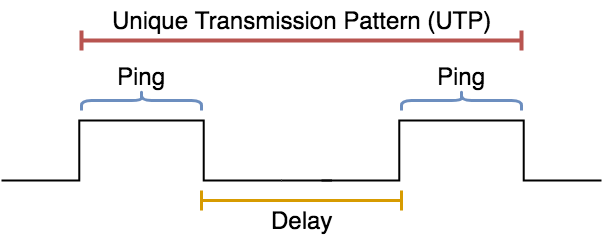
\includegraphics[scale=0.5]{utp}

\caption{A Unique Transmission Pattern}\label{fig:utp}
\end{figure}


%%%%%%%%%%%%%%%%%%%%%%%%%%%%%%%%%%%%%%%%%%%%%%%%%%%%%%%%%%%%%%%%%%%%%%%%%%%%%%%

\appendix
\section{Glossary of Terms} \label{glossary}

{\bf Delay:}
	in the context of ID encoding, the space between the falling edge of one
	{\bf ping} and the rising of the next within a single {\bf UTP}.

{\bf Delay Time ({\em d}):}
	the duration (generally in milliseconds) of a given {\bf delay}.

{\bf iCRAB (id-correlated rhythmic audio broadcast) protocol:}
	the protocol designed by the members of the Crab Tracker project and
	described in detail in this document.

{\bf Interval:}
	the time between two consecutive broadcasts of {\bf UTP}. Measured by the
	distance between the final falling edge of one ping and the first rising
	edge of the next.

{\bf Ping:}
	a single, continuous transmission of signal.

{\bf Ping Duration:}
	the length of time between the rising and falling edges of a continuous
	transmission (a {\bf ping}).

{\bf Unique Transmission Pattern, UTP:}
	a sequence of two {\bf ping}s separated by some {\bf delay} used to
	encode the unique identifier of a transmitter.

\end{document}

